% vim: set textwidth=78 autoindent:

\section{QGIS Plugins}\label{sec:plugins}\index{plugins}

% when the revision of a section has been finalized, 
% comment out the following line:
%\updatedisclaimer

QGIS has been designed with a plugin architecture.
This allows new features/functions to be easily added to the application.
Many of the features in QGIS are actually implemented as \textbf{core} or \textbf{external} plugins.\index{plugins!types} 

\begin{itemize}
\item \textbf{Core Plugins} are maintained by the QGIS Development Team and are automatically part of every QGIS distribution.
They are written in one of two languages: C++ or Python.
More information about core plugins are provided in Section \ref{sec:core_plugins}.
\item \textbf{External Plugins} are currently all written in Python.
They are stored in external repositories and maintained by the individual author.
They can be added to QGIS using the core plugin called \filename{Plugin Installer}.
More information about external plugins are provided in Section \ref{sec:external_plugins}.
\end{itemize}

\subsection{Managing Plugins}\label{sec:managing_plugins}
\index{plugins!managing} 

Managing plugins in general means loading or unloading them using the \filename{Plugin Manager} plugin.
External plugins need to be first installed using the \filename{Plugin Installer} plugin.

\subsubsection{Loading a QGIS Core Plugin}\label{sec:load_core_plugin} 

Loading a QGIS Core Plugin is provided in the main menu \mainmenuopt{Plugins} > \dropmenuopttwo{mActionShowPluginManager}{Manage Plugins...}.\index{plugins!manager}

\begin{figure}[ht]
   \begin{center}
   \caption{Plugin Manager \nixcaption}\label{fig:pluginmanager}\smallskip
   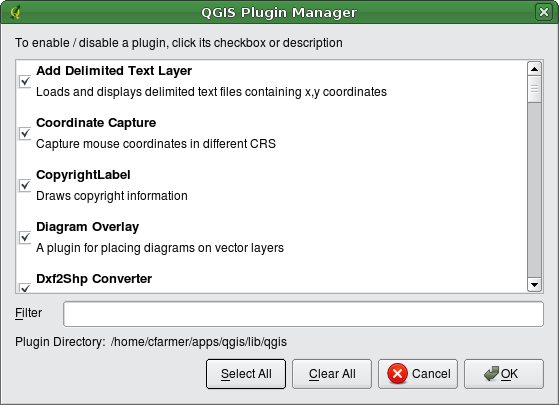
\includegraphics[clip=true, width=14cm]{pluginmanager}
\end{center}
\end{figure}

The Plugin Manager lists all the available plugins and their status (loaded or unloaded).
All available means all core plugins and all external plugins you added using \filename{Plugin Installer} plugin (see Section \ref{sec:external_plugins}). 
Figure \ref{fig:pluginmanager} shows the Plugin Manager dialog.
Loaded plugins are "remembered" when you exit the application and restored the next time you run QGIS.

\begin{Tip}\caption{\textsc{Crashing Plugins}}\index{crashes}
\qgistip{If you find that QGIS crashes on startup, a plugin may be at fault.
You can stop all plugins from loading by editing your stored settings file (see \ref{subsec:gui_options} for location).
Locate the plugins settings and change all the plugin values to false to prevent them from loading.
\nix {For example, to prevent the Delimited text plugin from loading, the entry in \$HOME/.config/QuantumGIS/qgis.conf on Linux should look like this:\usertext{Add Delimited Text Layer=false}.}
\normalfont 
Do this for each plugin in the [Plugins] section.
You can then start QGIS and add the plugins one at a time from the Plugin Manger to determine which is causing the problem.}
\end{Tip} 

\subsubsection{Loading an external QGIS Plugin}\label{sec:load_external_plugin} 

To be able to integrate external plugins into QGIS you first need to load the \filename{Plugin Installer} plugin as desribed in Section \ref{sec:load_core_plugin}.
Then you can load external QGIS python plugin in two steps: 

\begin{enumerate}
\item Download an external plugin from a repository using the \filename{Plugin Installer} (Section \ref{sec:python_plugin_installer}).
The new external plugin will be integrated into the list of available plugins in the \filename{Plugin Manager}.
\item Load the plugin using the \filename{Plugin Manager}.
\end{enumerate}

\subsubsection{Using the QGIS Python Plugin Installer}\index{plugins!installing}\label{sec:python_plugin_installer}
\index{plugins!Python Plugin Installer}\index{plugins!upgrading}

\begin{figure}[ht]
   \begin{center}
   \caption{Installing external python plugins \nixcaption}
\label{fig:plugininstaller}\smallskip
   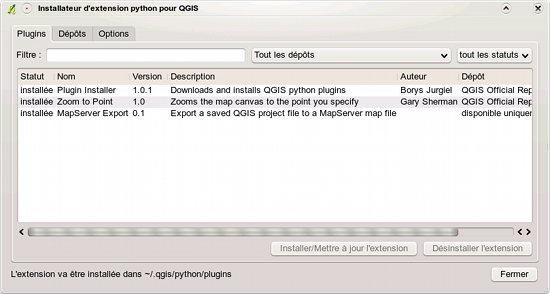
\includegraphics[clip=true, width=14cm]{plugininstaller}
\end{center}
\end{figure}

In order to download and install an external Python plugin, click the menu \mainmenuopt{Plugins} > \dropmenuopttwo{plugin_installer}{Fetch Python Plugins...}.
The \filename{Plugin Installer} window will appear (figure \ref{fig:plugininstaller}) with the tab \tab{Plugins}, containing the list of all Python plugins available in remote repositories as well as installed ones. Each plugin can be either:
\begin{itemize}
\item \textbf{not installed} - it means the plugin is available in the repository, but is not installed yet. In order to install, select it from the list and click the \button{Install plugin} button.
\item \textbf{new} - the same as before but the plugin is seen for the first time.
\item \textbf{installed} - the plugin is installed. If it's also available in any repository the \button{Reinstall plugin} button is enabled. But if the available version is older than the installed one, the \button{Downgrade plugin} button appears instead.
\item \textbf{upgradeable} - the plugin is installed, but there is an updated version available. The \button{Upgrade plugin} button is enabled.
\item \textbf{invalid} - the plugin is installed, but is unworkable. The reason is explained in the plugin description.
\end{itemize}

\minisec{Plugins tab}

To install a plugin, select it from the list and click the \button{Install plugin} button. The plugin is installed in its own directory, e.g. for \nix under \filename{\$HOME/.qgis/python/plugins} and is only visible for the user who has installed it. See a list of other OS specific subdirectory used for plugins in Section~\ref{subsec:pyfoursteps}. If the installation is successful, a confirmation message will appear. Then you need go to the \mainmenuopt{Plugins} > \dropmenuopttwo{mActionShowPluginManager}{Manage Plugins...} and load the installed plugin. 

If the installation fails, the reason is displayed. The most often troubles are related to connection errors and missing Python modules. In the former case you'll probably need to wait some minutes or hours, in the latter one you need to install the missing modules in your operating system prior to using the plugin. \nix{For Linux, most required modules should be available in a package manager}. \win{For install instructions in Windows visit the module home page}. If you use a proxy, you may need to configure it under the menu \mainmenuopt{Settings} > \dropmenuopttwo{mActionOptions}{Options} on the \tab{Proxy} tab.

The \button{Uninstall plugin} button is enabled only if the selected plugin is installed and it's not a core plugin. Note that if you have installed an update of a core plugin, you can still uninstall this update with the \button{Uninstall plugin} and revert to the version shipped within Quantum GIS install package. This one cannot be uninstalled.

\minisec{Repositories tab}

The second tab \tab{Repositories} contains a list of plugin repositories available for the Plugin Installer. By default, only the QGIS Official Repository is used. You can add some user-contributed repositories, including the central QGIS Contributed Repository and a few author repositories by clicking the \button{Add 3rd party repositories} button. Those repositories contain a huge number of more or less useful plugins but please note that they aren't maintained by the QGIS Development Team and we can't take any responsibility for them. You can also manage the repository list manually, that is add, remove and edit the entries. Temporary disabling a particular repository is possible clicking the \button{Edit...} button.

The \checkbox{Check for updates on startup} checkbox makes QGIS looking for plugin updates and news. If it's enabled, all repositories listed and enabled on the \tab{Repositories} tab are checked whenever the program is starting. If a new plugin or an update for one of installed plugins is available, a clickable notification appears in the Status Bar. If the checkbox is disabled, looking for updates and news is performed only when Plugin Installer is being launched from the menu.

In case of some internet connection problems a \textit{Looking for new plugins...} indicator in the Status Bar may stay visible during whole QGIS session and cause a program crash when exiting. In this case please disable the checkbox.

\subsection{Data Providers}\index{data providers}

Data Providers are "special" plugins that provides access to a data store.
By default, QGIS supports PostGIS layers and disk-based data stores supported by the GDAL/OGR library (Appendix \ref{appdx_ogr}).
A Data Provider plugin extends the ability of QGIS to use other data sources.

Data Provider plugins are registered automatically by QGIS at startup.
They are not managed by the Plugin Manager but used behind the scenes when a data type is added as a layer in QGIS.
